\chapter{Implementierung und Benchmarks}
Die verwendete Bibliothek wurde in der Vorlesung High Performance Computing 1 entwickelt \cite{HPC1}.

Die Bibliothek ist in C++ geschrieben. Es sind Klassen für Matrizen und Vektoren implementiert, sowie einige BLAS-Routinen.

Die Matrix-Klassen erlauben den zugriff auf Matrixblöcke. 



Eventuell Beispiel

\section{Aufwand}

Die QR-Zerlegung einer Matrix $A \in \mathbb{R}^{m \times n}$  erfordert
\begin{align*}
	n^2(m-\frac{1}{3} n) + {\cal O}(mn)
\end{align*}
Rechenoperationen.

\subsection{FLOPS}
FLPOS (Floating Point Operations Per Second) 

\section{Fehlerschätzer}

Es wurde der Fehlerschätzer von ATLAS\cite{atlas} verwendet.
\begin{align}
	err = \dfrac{\|A - QR\|_i}{\|A\|_i \cdot \min(m,n) \cdot \varepsilon}
\end{align}
$\|\cdot\|_i$ ist eine passende Norm.
Die Matrizen $Q$ und $R$ sind die QR-Zerlegung der Matrix $A \in \mathbb{R}^{m \times n}$.
$\varepsilon$ ist die kleinste darstellbare Zahl.\\
Die QR-Zerlegung ist gut genug falls der Fehler kleiner 1 ist $ err < 1 $.

Als Norm wurde die Zeilensummennorm $\|\cdot\|_\infty$ gewählt.
Diese ist für eine Matrix $A \in \mathbb{R}^{m\times n}$ gegeben durch
\begin{align*}
	\|A\|_\infty = \max_{i=1,...,m} \sum_{j=1}^{n} |a_{ij}|
\end{align*}

$\epsilon$ ist auf dem Test-System $2.220446\cdot10^{-16}$


\section{Benchmarks}

\subsection{Test System}

Getestet wurde auf einem System mit einer Intel(R) Core(TM) i5-3470 CPU mit 3.20GHz. 

Die Theoretische peak performance errechnet sich aus der Taktrate mal die Registerbreite mal 2.

Die CPU des Test Systems hat eine Taktrate von 3.20GHz.
Die AVX-Register sind 256-Bit groß. Darin haben 4 double Platz.

\begin{align*}
	\text{Taktrate} \cdot \text{Registerbreite} \cdot 2= 3,20 \text{ GHz} \cdot 4 \cdot 2 = 25,6 \text{ GFLOPs}
\end{align*}

\begin{figure}[H]
	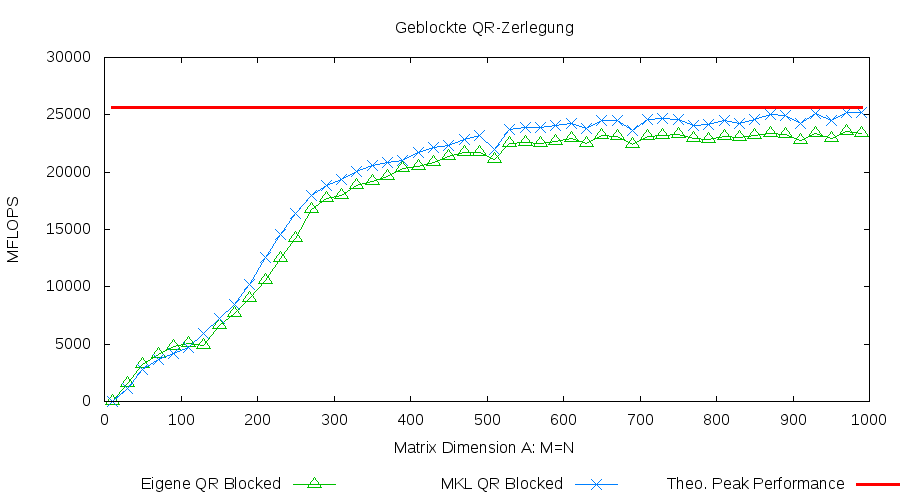
\includegraphics[width=\textwidth]{images/blk.png}
	\caption{Benchmark geblockte QR-Zerlegung}
	\label{img:blk}
\end{figure}

\begin{figure}[H]
	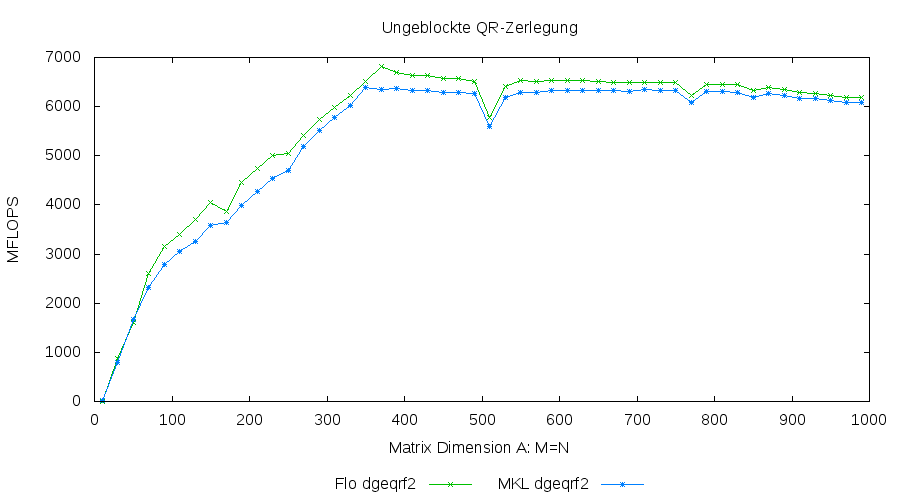
\includegraphics[width=\textwidth]{images/unblk.png}
	\caption{Benchmark ungeblockte QR-Zerlegung}
	\label{img:unblk}
\end{figure}








	 